% \documentclass{article}
% \usepackage{beamerarticle}
\documentclass{beamer}
% Beamer theme settings
\usetheme{Madrid}
\usecolortheme{default}
\usepackage{amsmath}
\usepackage{tikz}
\usetikzlibrary{intersections}
\usepackage{graphicx}

% Define commands for vectors
\newcommand{\va}{\mathbf{a}}
\newcommand{\vb}{\mathbf{b}}
\newcommand{\vc}{\mathbf{c}}
\newcommand{\vd}{\mathbf{d}}
\newcommand{\ve}{\mathbf{e}}
\newcommand{\vv}{\mathbf{v}}
\newcommand{\vu}{\mathbf{u}}
\newcommand{\vw}{\mathbf{w}}
\newcommand{\vx}{\mathbf{x}}
\newcommand{\vy}{\mathbf{y}}
\newcommand{\vz}{\mathbf{z}}
\newcommand{\N}{\mathbb{N}}
\newcommand{\Z}{\mathbb{Z}}
\newcommand{\R}{\mathbb{R}}
\newcommand{\Q}{\mathbb{Q}}







% Title page

\title[Lecture 3]{Inverse, Determinant}
\author[Aprikyan, Tarkhanyan]{Hayk Aprikyan, Hayk Tarkhanyan}
% \institute[ACA]{Armenian Code Academy}
\date{March 25, 2025}

\begin{document}

\begin{frame}
  \titlepage
\end{frame}

%%%%%%%%%%%%%%% Berel em naxordic


% % Slide 0: linear comb
% \begin{frame}{Linear Combination}
% Note that \textit{if $\vv_1,\dots,\vv_k$ were numbers} we could also denote $\mathbf{c} = \begin{bmatrix}
%     c_1\\c_2\\\vdots\\c_k
% \end{bmatrix}$, $\mathbf{v^*} = \begin{bmatrix}
%     \vv_1\\\vv_2\\\vdots\\\vv_k
% \end{bmatrix}$ and the linear combination could be written in the form:
% \[c_1\mathbf{v}_1 + c_2\mathbf{v}_2 + \ldots + c_k\mathbf{v}_k = \vc \cdot \mathbf{v^*}= \mathbf{v^*}\cdot \vc\]

% \pause But what to do when $\vv_1,\dots,\vv_k$ are vectors?
% \end{frame}

% % %%%%%%%%%%%%%%%%%%%%%%%%%%%%%%%

% % Slide 4: I
% \begin{frame}
%   \frametitle{Inverse Matrix}
%   Let's get back to dot products of vectors. Let $\vv \in \R^n$ be some vector. Which vector should we multiply $\vv$ by to get 1?
%   \pause The answer is $\frac{\vv}{\|\vv\|^2}$:
  
% \[      \mathbf{v} \cdot \frac{\mathbf{v}}{\|\mathbf{v}\|^2} = \frac{\mathbf{v} \cdot \mathbf{v}}{\|\mathbf{v}\|^2} = \frac{v_1^2 + v_2^2+\dots+v_n^2}{v_1^2 + v_2^2+\dots+v_n^2}=1
% \]

% (because $\|\vv\|=\sqrt{\vv \cdot \vv}$).

% \pause How about matrices? What should we multiply a matrix with, to get the unit matrix?

% \end{frame}





% slide 6: definite
\begin{frame}{Geometric Interpretation }

\textbf{Recap:}

When you multiply, say, a $2\times 2$ matrix $A$ by a vector $\vv\in\R^2$, what you get is another vector $\vu=A\vv\in\R^2$. We call this $\vu$ the \textbf{transformed version} of $\vv$ (and we say that $A$ is a linear transformation).

\begin{figure}
    \centering
    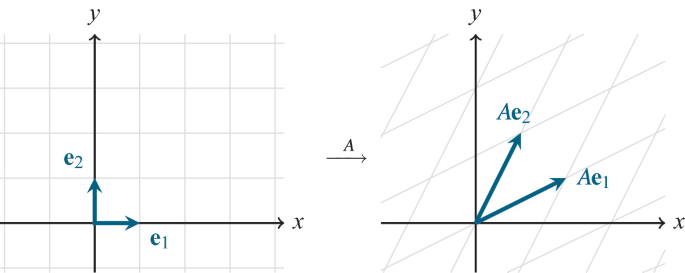
\includegraphics[width=0.75\linewidth]{viz ex.png}
    
    
\end{figure}

\end{frame}


% slide 6: definite
\begin{frame}{Geometric Interpretation }

As we will see later, the resulting "transformed version" $\vu$ is just the same old $\vv$ except it is \textbf{rotated} and \textbf{scaled} to become longer or shorter (and possibly, flipped).

\pause 

\bigskip

In this sense, all  matrices are either just rotating vectors by some degree, or flipping them horizontally/vertically, or scale them, or do all three.

\smallskip 

The key thing is: whatever a matrix "does" to one vector, it does the same to all other vectors too (when being multiplied with them).

\bigskip
\bigskip


{\small
\textcolor{blue}{Check different matrices yourself:\\ - \url{visualize-it.github.io/linear_transformations/simulation.html} 
\\ - \url{www.shad.io/MatVis}
}}

\pause 

\bigskip 


Now that we know what matrix $\times$ vector multiplication means,  
what about matrix $\times$ matrix multiplication? Why is it defined the way it is?

    
\end{frame}






\begin{frame}{Geometric Interpretation }

Suppose $\mathbf{v} \in \R^2$, $A \in \R^{2 \times 2}$, $B \in \R^{2 \times 2}$:

\begin{figure}
    \centering
    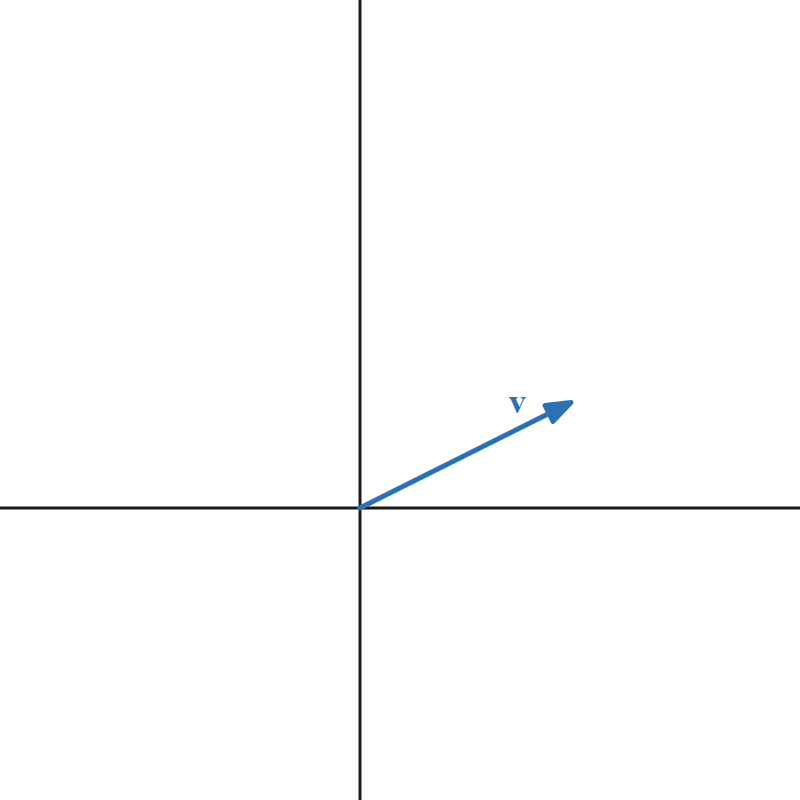
\includegraphics[width=0.5\linewidth]{matrix product/desmos-graph (1).png}
\end{figure}
\end{frame}


\begin{frame}{Geometric Interpretation }

If we apply $A$ on $\mathbf{v} $, we get a transformed version of $\mathbf{v} $,

\begin{figure}
    \centering
    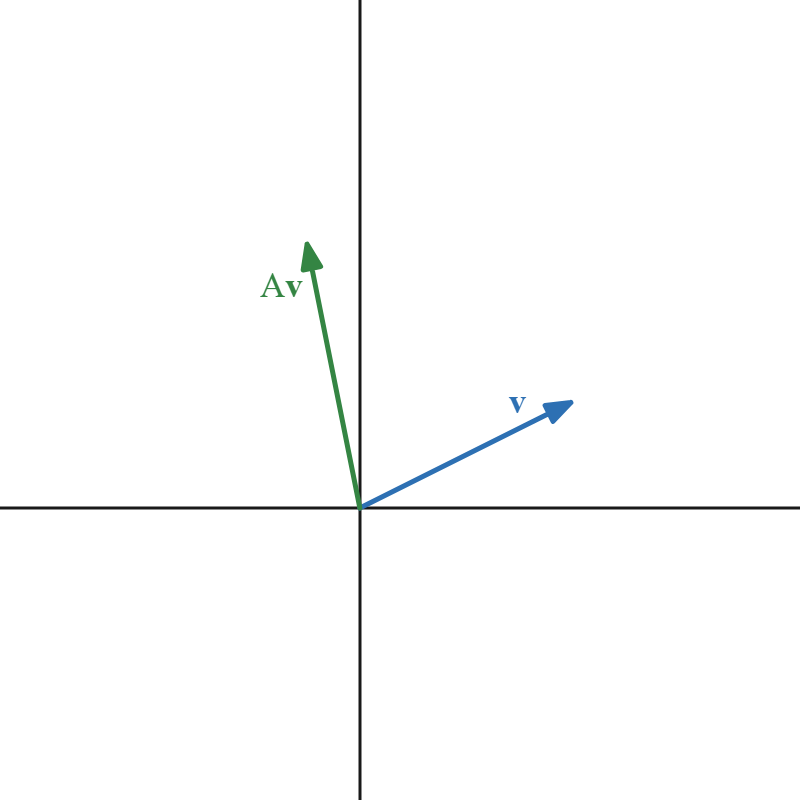
\includegraphics[width=0.5\linewidth]{matrix product/desmos-graph (2).png}
\end{figure}



    
\end{frame}



\begin{frame}{Geometric Interpretation }

If we apply $A$ on $\mathbf{v} $, we get a transformed version of $\mathbf{v} $, say $\mathbf{u}$:

\begin{figure}
    \centering
    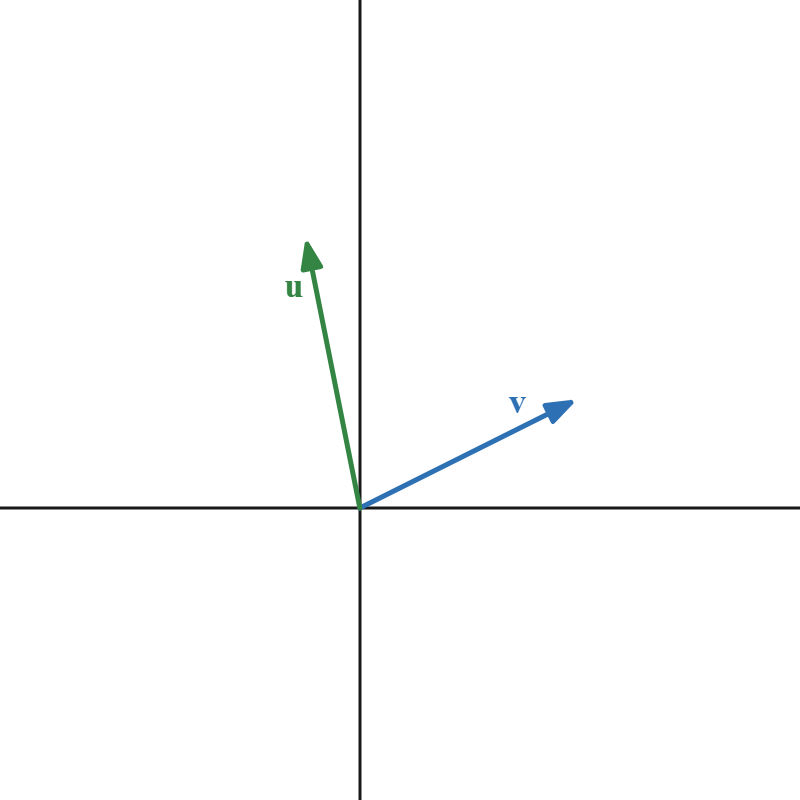
\includegraphics[width=0.5\linewidth]{matrix product/desmos-graph (3).png}
\end{figure}    
\end{frame}



\begin{frame}{Geometric Interpretation }

Now  applying $B$ on $\mathbf{u} $, we get a  transformed version of $\mathbf{u} $, i.e. $B\mathbf{u}$

\begin{figure}
    \centering
    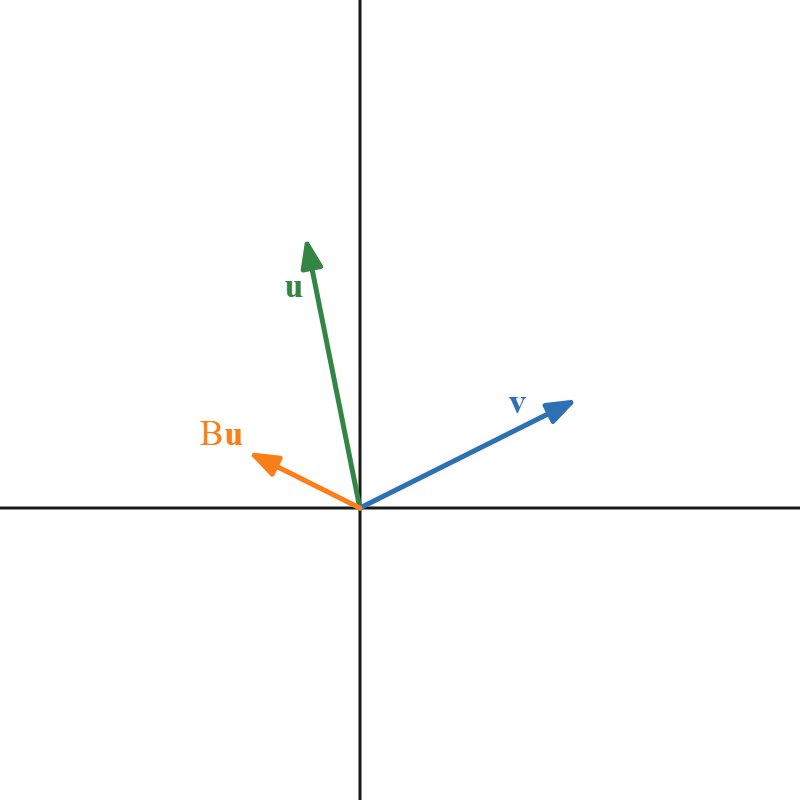
\includegraphics[width=0.5\linewidth]{matrix product/desmos-graph (4).png}
\end{figure}    
\end{frame}

\begin{frame}{Geometric Interpretation }

Now  applying $B$ on $\mathbf{u} $, we get a  transformed version of $\mathbf{u} $, i.e. $B\mathbf{u}=BA\mathbf{v}$

\begin{figure}
    \centering
    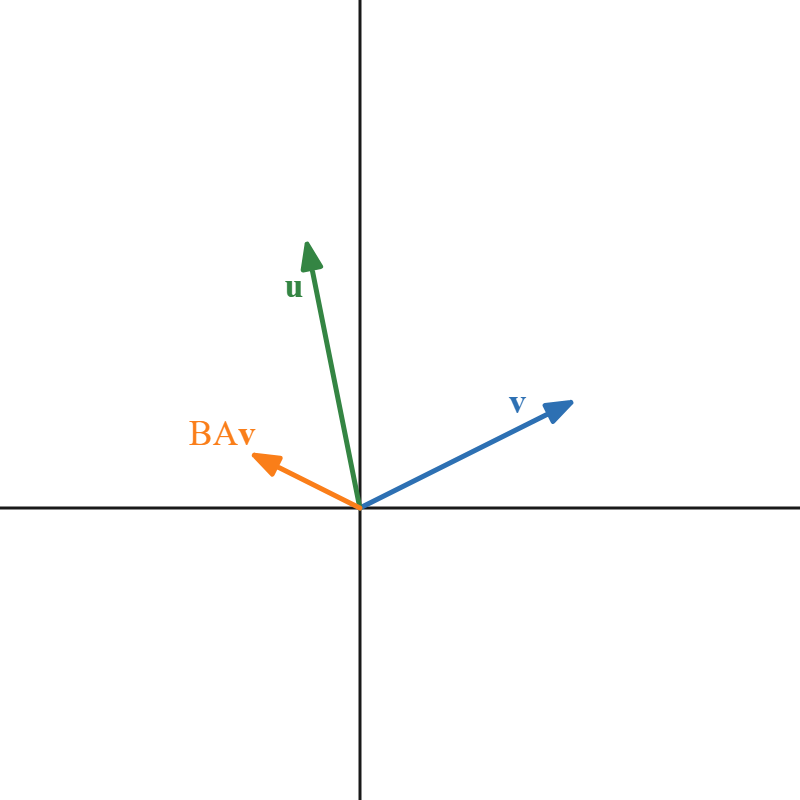
\includegraphics[width=0.5\linewidth]{matrix product/desmos-graph (5).png}
\end{figure}    
\end{frame}


\begin{frame}{Geometric Interpretation }

So what is the product $BA$? To get $(BA)(\mathbf{v})$, we do:

\begin{figure}
    \centering
    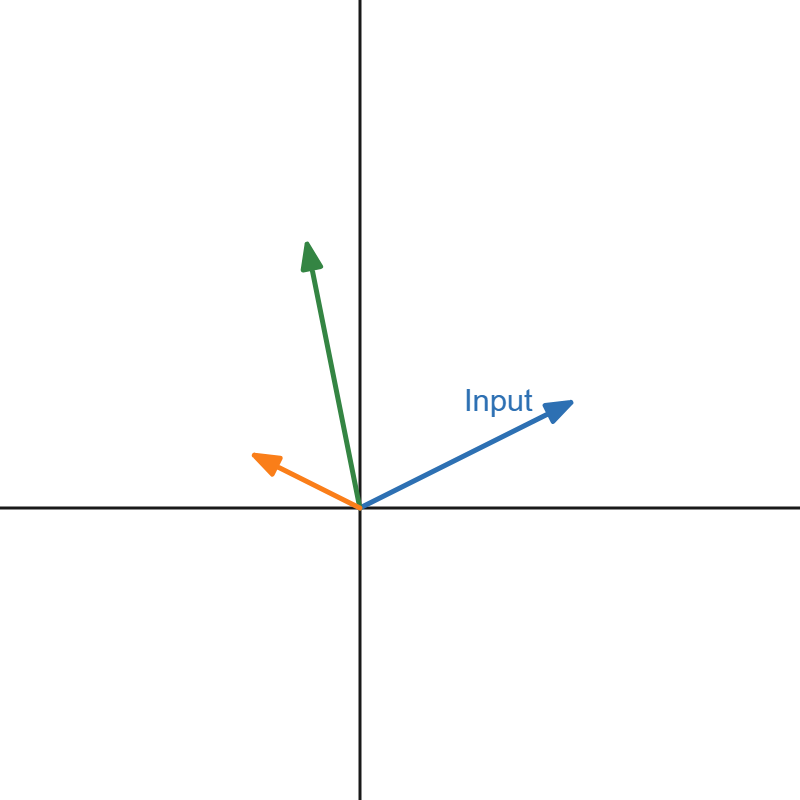
\includegraphics[width=0.5\linewidth]{matrix product/desmos-graph (6).png}
\end{figure}    
\end{frame}

\begin{frame}{Geometric Interpretation }

So what is the product $BA$? To get $(BA)(\mathbf{v})$, we do:

\begin{figure}
    \centering
    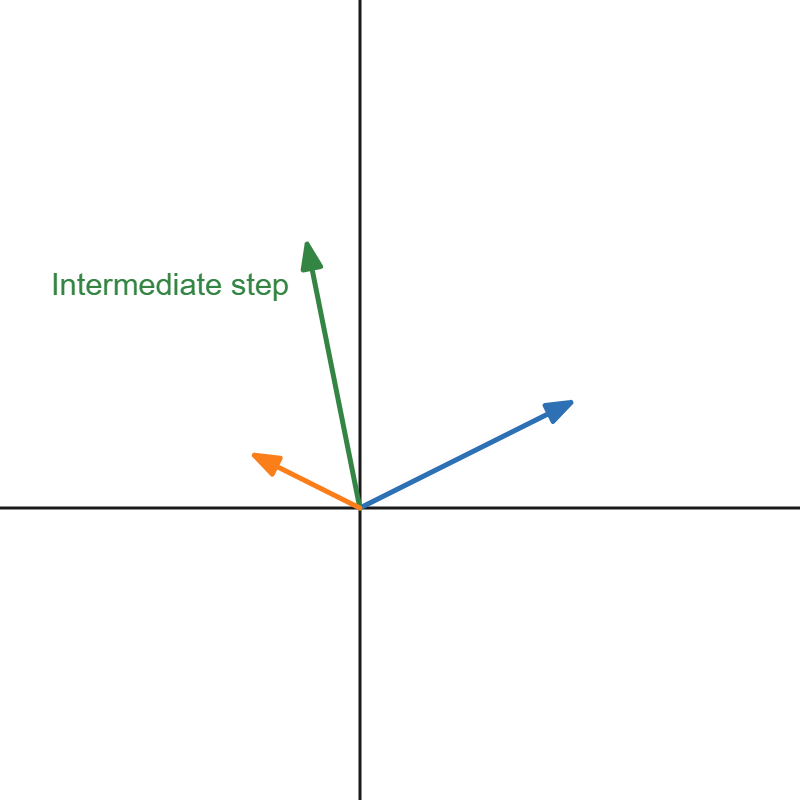
\includegraphics[width=0.5\linewidth]{matrix product/desmos-graph (7).png}
\end{figure}    
\end{frame}

\begin{frame}{Geometric Interpretation }

So what is the product $BA$? To get $(BA)(\mathbf{v})$, we do:

\begin{figure}
    \centering
    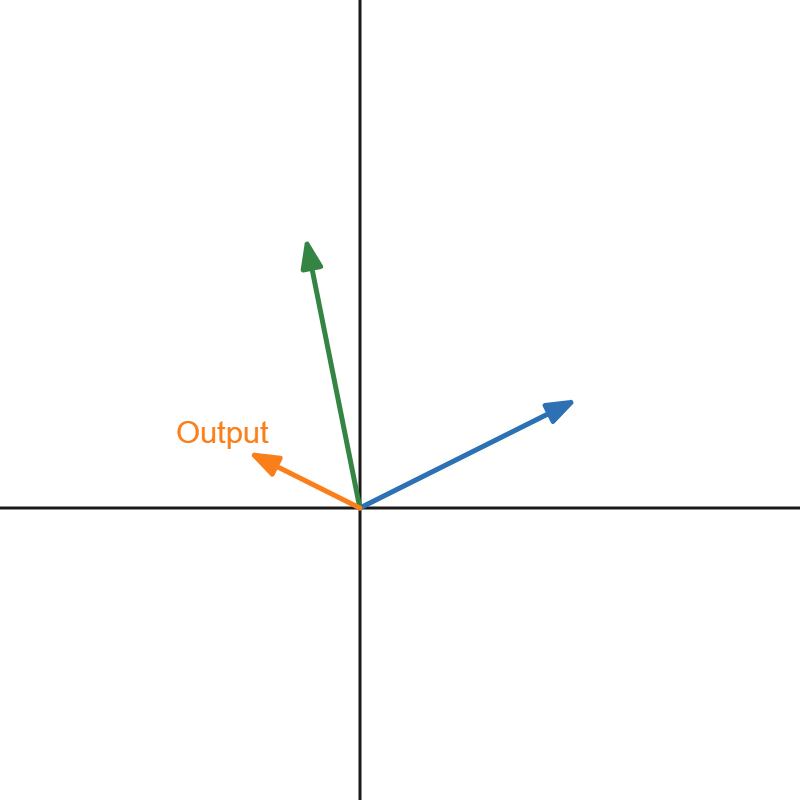
\includegraphics[width=0.5\linewidth]{matrix product/desmos-graph (8).png}
\end{figure}    
\end{frame}

\begin{frame}{Geometric Interpretation }

Hence $BA$ is the linear transformation that we get by \textbf{first applying $A$}, and \textbf{then applying $B$}!

\pause

(Note that this means that often $AB$ is \textit{not the same} as $BA$)

\pause


\bigskip

\begin{block}{Question}
    Suppose $A$ is the matrix that rotates the vectors by $30^\circ$,  $B$ the one that rotates by $50^\circ$, and $C$ by $260^\circ$.

    \pause

    What would the product matrix $BA$ be? \pause 
    What about $CBA$?
\end{block}

\bigskip

\pause

Which matrix leaves everything in its place (does not touch anything)?

\end{frame}








% Slide 4: I
\begin{frame}
  \frametitle{Identity Matrix}


  \begin{block}{Definition}
    A matrix is said to be \textbf{square} if it has the same number of rows and columns. In other words, an \(n \times n\) matrix is a square matrix.
  \end{block}

  \pause
  \begin{block}{Definition}
    A square matrix \(A\) is \textbf{symmetric} if \(A^T = A\), i.e., the transpose of \(A\) is equal to \(A\).
  \end{block}

  \pause


  \begin{example}
    \[
      A = \begin{bmatrix}
        2 & 0 & 1 \\
        0 & -3 & 4 \\
        1 & 4 & 6 \\
      \end{bmatrix}
    \]
    This matrix is both symmetric and (of course) square.
  \end{example}
\end{frame}
\begin{frame}
  \frametitle{Identity Matrix}


  \begin{block}{Definition}
    The \textbf{main diagonal} (or just the \textbf{diagonal}) of a matrix $A$ are the terms $a_{ii}$ for which the row and column indices are the same ($a_{11}$, $a_{22}$, $\dots$), so from the upper left element to the lower right.
  \end{block}

  \pause

  Similarly, the other diagonal from the upper right element to the lower left is called the \textbf{secondary diagonal}.

  \pause

  \begin{figure}
      \centering
      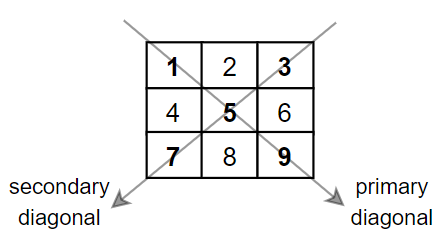
\includegraphics[width=0.5\linewidth]{twodiagonals.png}
      
      
  \end{figure}

\end{frame}



\begin{frame}
  \frametitle{Identity Matrix}
% \begin{example}
    For example, here the main diagonal is marked with red:
\begin{figure}
    \centering
    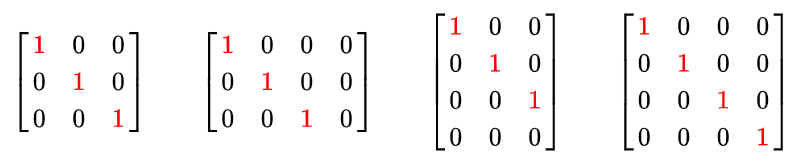
\includegraphics[width=\linewidth]{diagonals.png}    
\end{figure}
\pause
The secondary diagonal is marked with red:
\begin{figure}
    \centering
    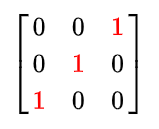
\includegraphics[width=0.2\linewidth]{image.png}
\end{figure}
% \end{example}

\end{frame}



\begin{frame}
  \frametitle{Identity Matrix}


  \begin{block}{Definition}
    The \textbf{identity matrix} of $\R^{n \times n}$, denoted as \(I_n\), is the square matrix with ones on the main diagonal and zeros elsewhere.
  \end{block}

Applying the identity matrix on vectors does not change them.

  \pause

  \begin{example}
    \[
      I_3 = \begin{bmatrix}
        1 & 0 &0  \\
        0 & 1 &0\\
        0 &0& 1\\
      \end{bmatrix}
    \text{  is the $3\times 3$ identity matrix.}\]
    
  \end{example}
\pause

Therefore, we can say:
\begin{block}{Property}
    For any matrix $A\in\R^{m\times n}$,
    \[ I_m A = A I_n = A\]
\end{block}

\end{frame}





\begin{frame}
  \frametitle{Inverse Matrix}

Finally, what if we have a vector in $\R^n$,

\begin{figure}
    \centering
    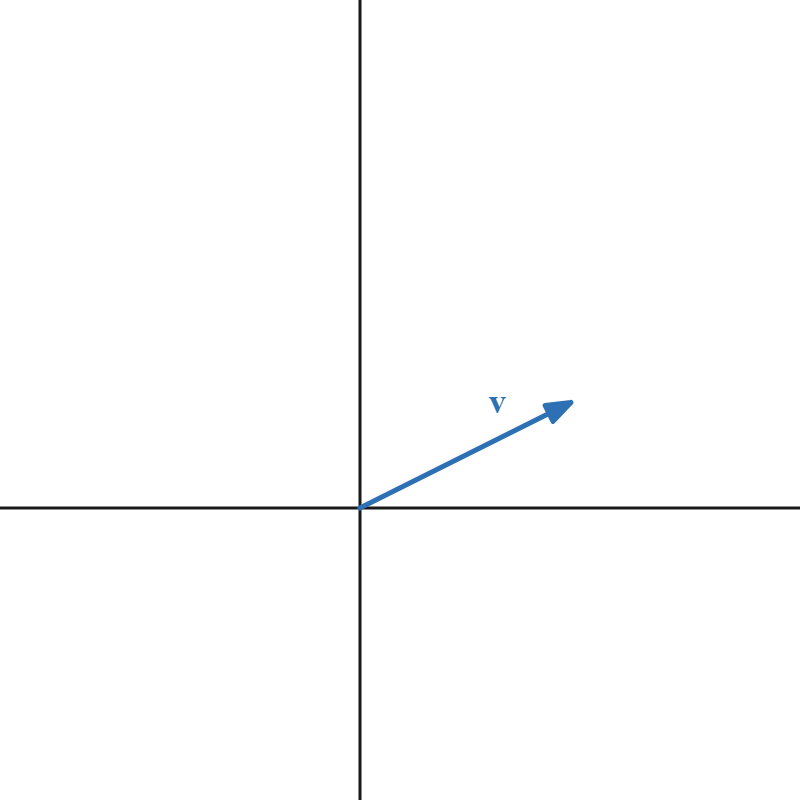
\includegraphics[width=0.5\linewidth]{matrix product/desmos-graph (9).png}
\end{figure}    
\end{frame}


\begin{frame}
  \frametitle{Inverse Matrix}

Finally, what if we have a vector in $\R^n$, and we accidentally transform it?

\begin{figure}
    \centering
    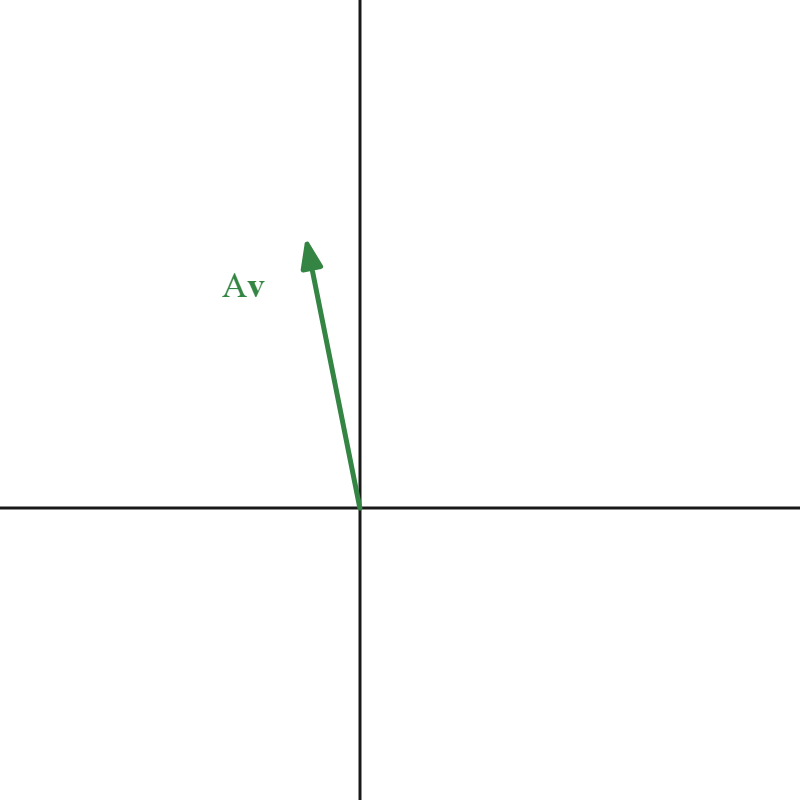
\includegraphics[width=0.5\linewidth]{matrix product/desmos-graph (10).png}
\end{figure}    
\end{frame}

\begin{frame}
  \frametitle{Inverse Matrix}

How to get back to the original vector?

\begin{figure}
    \centering
    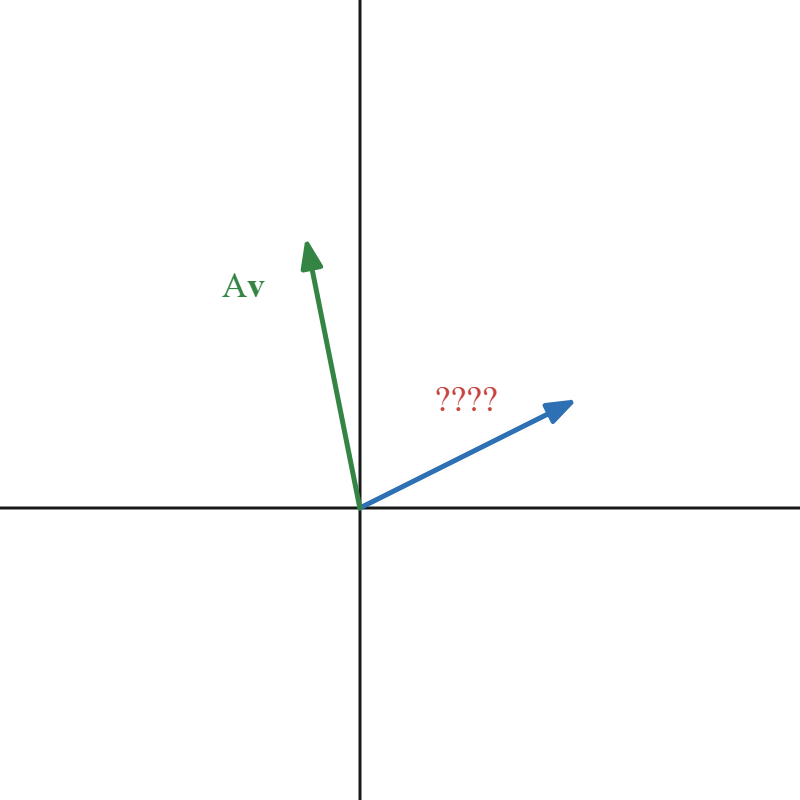
\includegraphics[width=0.5\linewidth]{matrix product/desmos-graph (11).png}
\end{figure}    
\end{frame}


\begin{frame}
  \frametitle{Inverse Matrix}

In other words, in terms of what we learned about matrix multiplication, 
\[
\textbf{what} \times A = I \quad ?
\]

\pause

We call that matrix the \textbf{inverse} of $A$, and we denote it by $A^{-1}$.

\end{frame}


\begin{frame}
  \frametitle{Inverse Matrix}

In other words, in terms of what we learned about matrix multiplication, 
\[
A^{-1} \times A = I \quad !
\]



We call that matrix the \textbf{inverse} of $A$, and we denote it by $A^{-1}$.

\end{frame}



\begin{frame}
  \frametitle{Inverse Matrix}

\begin{block}{Question}
    Assume the matrix $A \in \R^{n \times n}$ does the following when applied on a vector:

    \begin{enumerate}
        \item scales the vector up $2$ times in the horizontal direction, 
        \item then rotates it by $30^\circ$ clockwise,
        \item then squishes it down $3$ times in the vertical direction,
        \item and then flips it horizontally (around the $x$-axis) $\sim$
    \end{enumerate}

\pause

Given $\mathbf{v}=A\mathbf{u}$, could we recover the original $\mathbf{u}$?
    
\end{block}

\pause

The answer is yes, i.e. the matrix $A$ has an inverse. As we will see soon, only some square matrices actually have an inverse.

\end{frame}


% slide: trace
\begin{frame}
  \frametitle{Trace }

  \begin{block}{Definition}
    The \textbf{trace} of a square matrix \(A\), denoted as \(\text{tr}(A)\), is the sum of the elements on its main diagonal.
    \[
      \text{tr}(A) = a_{11} + a_{22} + \ldots + a_{nn}
    \]
  \end{block}

  \pause

  \begin{example}
    If
    \[
      A = \begin{bmatrix}
        2 & 5 & 1 \\
        0 & -3 & 4 \\
        7 & 2 & 6 \\
      \end{bmatrix}
    \]
    then
    \[
      \text{tr}(A) = 2 + (-3) + 6 = 5
    \]
  \end{example}
\pause Note that only square matrices have a trace. 
\end{frame}


% slide: trace
\begin{frame}
  \frametitle{Trace }

  \begin{block}{Trace Properties}
    For any matrices \(A\) and \(B\), and any scalar \(c\), the trace of a matrix satisfies the following properties:

    \begin{itemize}
      \item \(\text{tr}(cA) = c \cdot \text{tr}(A)\)
      \item \(\text{tr}(A + B) = \text{tr}(A) + \text{tr}(B)\)
      \item \(\text{tr}(AB) = \text{tr}(BA)\) 
      \item \(\text{tr}(A^T) = \text{tr}(A)\)
    \end{itemize}
  \end{block}
\end{frame}


% slide: det
\begin{frame}
  \frametitle{Determinant of a \(2 \times 2\) Matrix}

  \begin{block}{Determinant Formula}
    For a \(2 \times 2\) matrix
    \[
      A = \begin{bmatrix}
        a & b \\
        c & d \\
      \end{bmatrix}
    \]
    the determinant is given by
    \[
      \text{det}(A) = ad - bc
    \]
  \end{block}

  \pause

  \begin{example}
    For the matrix
    \[
      A = \begin{bmatrix}
        2 & 5 \\
        -3 & 4 \\
      \end{bmatrix}
    \]
    the determinant is \(\text{det}(A) = (2)(4) - (5)(-3) = 8+15=23\).
  \end{example}

\end{frame}

% \begin{frame}
%   \frametitle{Determinant of a \(3 \times 3\) Matrix}

%   \begin{block}{Determinant Formula}
%      For a \(3 \times 3\) matrix
%     \[
%       C = \begin{bmatrix}
%         a & b & c \\
%         d & e & f \\
%         g & h & i \\
%       \end{bmatrix}
%     \]
%     the determinant is given by
%     \[
%       \text{det}(C) = aei + bfg + cdh - ceg - bdi - afh
%     \]
%   \end{block}

%   \pause

%   \begin{example}
%     For the matrix
%     \[
%       C = \begin{bmatrix}
%         1 & 2 & 3 \\
%         4 & 5 & 6 \\
%         7 & 8 & 9 \\
%       \end{bmatrix}
%     \]
%     \[
%       \text{det}(C) = 1\cdot5 \cdot 9 + 2\cdot6\cdot7 + 3\cdot4\cdot8-3\cdot5\cdot7-2\cdot4\cdot9-1\cdot6\cdot8= 0
%     \]
%   \end{example}


% \end{frame}

% \begin{frame}
%   \frametitle{Determinant of a \(3 \times 3\) Matrix}

%   \begin{center}
%     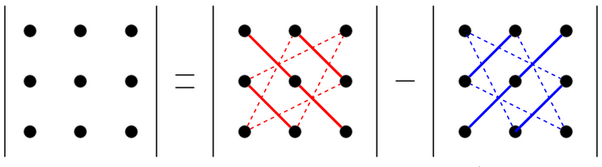
\includegraphics[width=\textwidth, height=\textheight, keepaspectratio]{det.png}
%   \end{center}
%   \end{frame}

\begin{frame}
  \frametitle{Determinant of a \(3 \times 3\) Matrix}

  \begin{block}{Determinant Formula}
     For a \(3 \times 3\) matrix
    \[
      C = \begin{bmatrix}
        a & b & c \\
        d & e & f \\
        g & h & i \\
      \end{bmatrix}
    \]
    the determinant is given by
    \[
      \text{det}(C) = aei + bfg + cdh - ceg - bdi - afh
    \]
  \end{block}

  \pause

\textbf{Forget that formula--remember the algorithm!}


\end{frame}

\begin{frame}
  \frametitle{Determinant of a \(3 \times 3\) Matrix}

  \begin{center}
    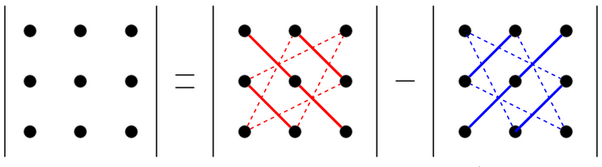
\includegraphics[width=\textwidth, height=\textheight, keepaspectratio]{det.png}
  \end{center}
  \end{frame}


\begin{frame}
  \frametitle{Determinant of a \(3 \times 3\) Matrix}
 Alternatively,
  \begin{center}
    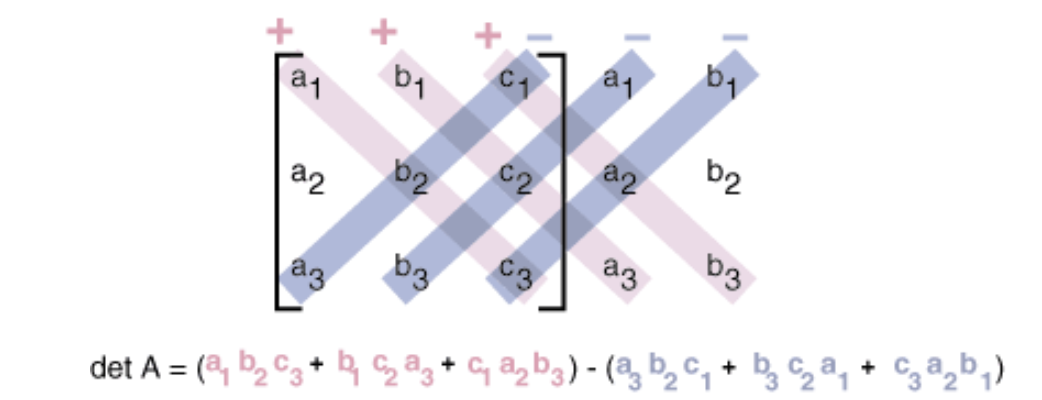
\includegraphics[width=\textwidth]{det_3_3.png}
  \end{center}
  \end{frame}


\begin{frame}
  \frametitle{Determinant of a \(3 \times 3\) Matrix}

  \begin{example}
    For the matrix
    \[
      C = \begin{bmatrix}
        1 & 2 & 3 \\
        4 & 5 & 6 \\
        7 & 8 & 9 \\
      \end{bmatrix}
    \]
    \[
      \text{det}(C) = 1\cdot5 \cdot 9 + 2\cdot6\cdot7 + 3\cdot4\cdot8-3\cdot5\cdot7-2\cdot4\cdot9-1\cdot6\cdot8= 0
    \]
  \end{example}

\pause

But what does the determinant show, and how do we need it?


  \end{frame}



% % esqan masy jnjel

% \begin{frame}{Determinant}

%   \begin{block}{Cofactors}
%     For a square matrix \(A\), the \textbf{cofactor} \(C_{ij}\) of the element \(a_{ij}\) is given by
%     \[
%       C_{ij} = (-1)^{i+j} \cdot \text{det}A_{ij}
%     \]
%     where \(A_{ij}\) is the matrix obtained by removing the \(i\)-th row and \(j\)-th column.
%   \end{block}

%   \pause


%   \begin{example}
%     For the matrix
%     \[
%       A = \begin{bmatrix}
%         2 & 1 \\
%         -3 & 4 \\
%       \end{bmatrix}
%     \]
%     the cofactors are \(C_{11} = 4\), \(C_{12} = -3\), and \(\text{det}(A) = 2 \cdot 4 + 1 \cdot 3 = 11\).
%   \end{example}

% \end{frame}


% \begin{frame}{Determinant}
%  \begin{example}
%     For the matrix
%     \[
%       A = \begin{bmatrix}
%         3 & 2 & 0\\
%         2 & 1 & -4\\
%         -1 & 5 & -3\\
%       \end{bmatrix}
%     \]
%     the cofactors of the elements on the first row ($[3,2,0]$) are: 
%     \[C_{11} = 1\cdot \bigg|\begin{array}{cc}1&-4\\5&-3\end{array}\bigg| = 17,\]
%     \[ C_{12}= (-1)\cdot \bigg|\begin{array}{cc}2&-4\\-1&-3\end{array}\bigg| = 2,\]
%     \[ C_{13}= 1\cdot\bigg|\begin{array}{cc}2&1\\-1&5\end{array}\bigg| = 11.\]
%     % and \(\text{det}(A) = 2 \cdot 4 + 1 \cdot 3 = 11\).
%   \end{example}
% \end{frame}



% \begin{frame}{Determinant}
    
%   \begin{block}{Determinant with Cofactors}
%     The determinant of a matrix \(A\) can be calculated using the cofactors:
%     \[
%       \text{det}(A) = a_{i1}C_{i1} + a_{i2}C_{i2} + \ldots + a_{in}C_{in}, \text{ for any }1\le i\le n \text{ (by row)}
%     \]    \[\text{or, equivalently,}\]\[
%       \text{det}(A) = a_{1i}C_{i1} + a_{2i}C_{i2} + \ldots + a_{ni}C_{in}, \text{ for any }1\le i\le n \text{ (by column)}
%     \]
%   \end{block}

%   \pause
%   \begin{example}
      
%     % Consider the matrix
%     \[
%       A = \begin{bmatrix}
%         1 & 2 & 3 & 4 \\
%         0 & 1 & 2 & 3 \\
%         1 & 0 & 1 & 2 \\
%         2 & 1 & 0 & 1 \\
%       \end{bmatrix}
%     \]
%     % Let's calculate the determinant of \(A\).
%     \[
%       \text{det}(A) = 1 \cdot \text{det}(A_{11}) - 2 \cdot \text{det}(A_{12}) + 3 \cdot \text{det}(A_{13}) - 4 \cdot \text{det}(A_{14})
%     \]
%     where \(A_{ij}\) is obtained by removing the \(i\)-th row and \(j\)-th column.
%   \end{example}

% \end{frame}

\begin{frame}{Determinant}

 If we take, for example, the so-called "unit square" formed by the vectors $\ve_1=[1\,\,\,\,0]$ and $\ve_2=[0\,\,\,\,1]$, we can see that their transformed versions, $A\ve_1$ and $A\ve_2$, form a parallelogram:

\begin{figure}
    \centering
    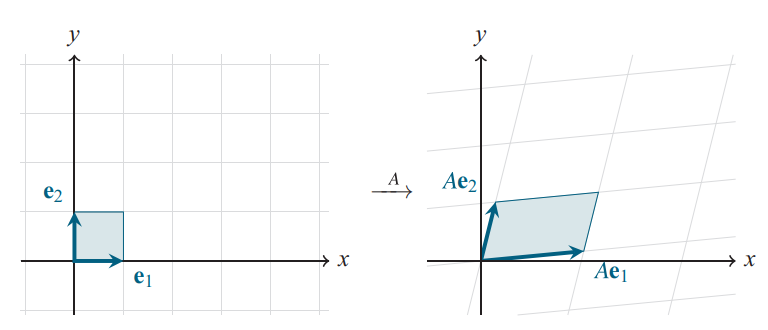
\includegraphics[width=0.75\linewidth]{viz det.png}
    
    
\end{figure}

\pause Then $\det(A)$ is  the area of that parallelogram.
\end{frame}



% slide 6: definite
\begin{frame}{Determinant}

More generally, after we apply the transformation $A$ (play that animation in your head), the area of \textit{any shape} gets scaled by the factor of $\det(A)$:

\begin{figure}
    \centering
    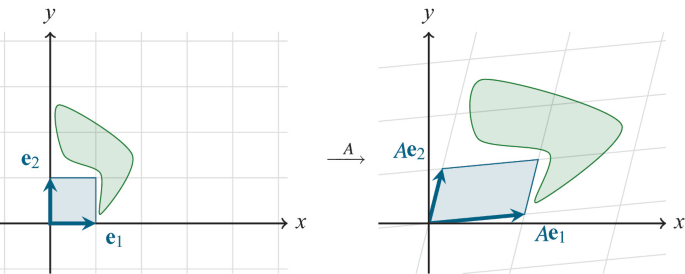
\includegraphics[width=0.75\linewidth]{viz area.png}
    
    
\end{figure}
\pause

 So the determinant shows how much the matrix scales up everything in average. Note that it is defined \textbf{only} for square matrices. 
\end{frame}


\begin{frame}{Determinant}
    
  \begin{block}{Determinant Properties}
    Let \(A, B\in\R^{n\times n}\) be square matrices of the same size, and let \(c\in\R\) be any scalar. Then:

    \begin{itemize}
      \item \(\text{det}(cA) = c^n \cdot \text{det}(A)\) \textit{(where \(n\) is the size of the matrix)}
      \item \(\text{det}(AB) = \text{det}(A) \cdot \text{det}(B)\) \textit{(multiplicativity)}
      \item $\det(I)=1$
\item If \(A\) is invertible, then \(\text{det}(A^{-1}) = \frac{1}{\text{det}(A)}\)
      \item \(\text{det}(A^T) = \text{det}(A)\) \textit{(invariance under transpose)}
      \item If all numbers on some row or some column of $A$ are zero, then $\det(A)=0$
       \item If $\det (A) <0$, then $A$ flips the space around.
    \end{itemize}
  \end{block}

  \pause

It would be an exercise of huge importance 
  to attempt proving these properties (except the last three) by playing the matrices in your head. 
\end{frame}




\begin{frame}{Determinant}

Finally,

\begin{block}{Question}
    What does it mean if $\det A = 0$?
\end{block}

\pause

\begin{figure}
    \centering
    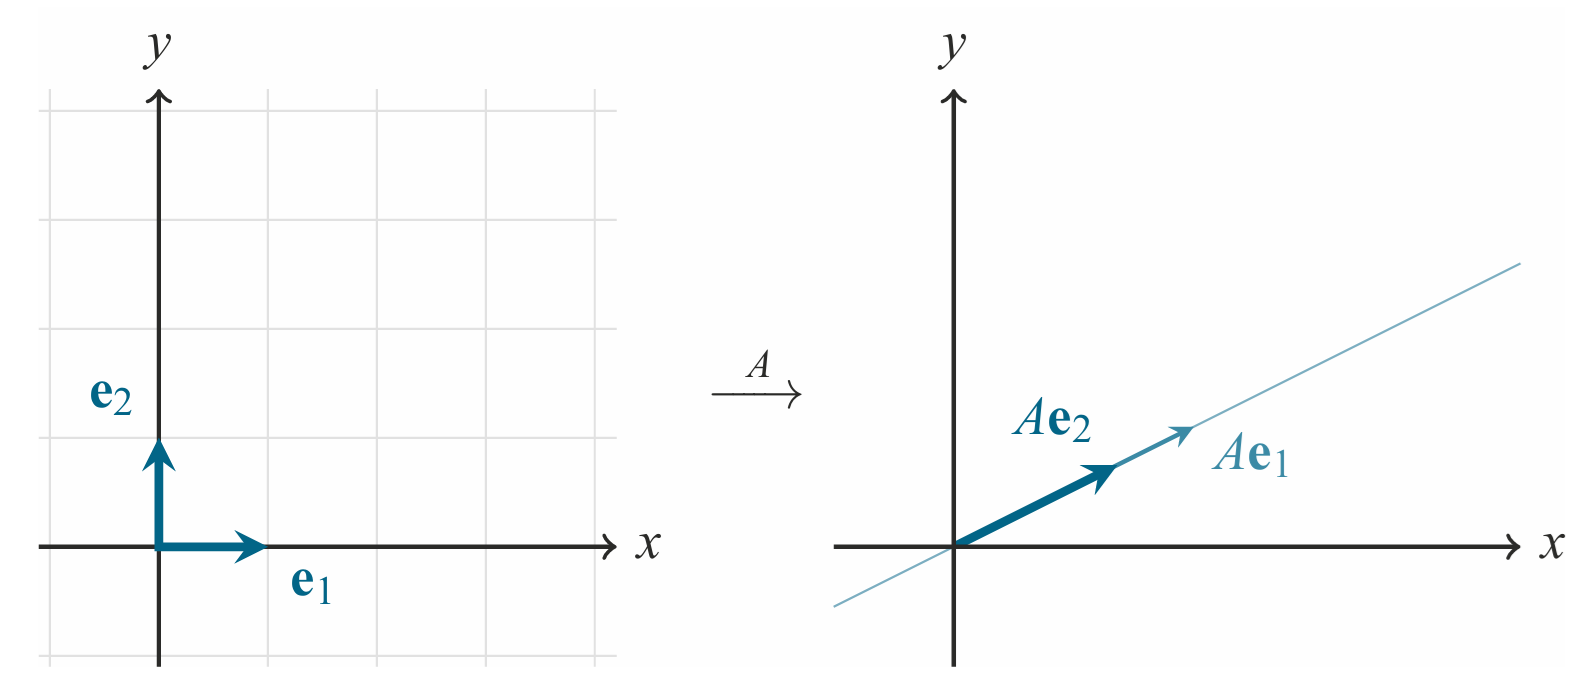
\includegraphics[width=0.85\linewidth]{0 det.png}
\end{figure}

% \begin{block}{Definition}
%     We say that a square matrix $A$ is \textbf{invertible} or \textbf{non-singular} if it has an inverse, i.e. there is a matrix $A^{-1}$,  such that $A  A^{-1} = A^{-1}  A = I$.
% \end{block}  
\pause
\begin{block}{Theorem}
  A square matrix $A$ has an inverse if and only if its determinant is not zero.
\end{block}  



\end{frame}
\begin{frame}{Inverse Matrix}
    \begin{block}{Formula for 2x2}
        For a $2 \times 2$ invertible matrix $A = \begin{bmatrix} a & b \\ c & d \end{bmatrix}$, the inverse $A^{-1}$ can be calculated using the formula:
      \[
      A^{-1} = \frac{1}{ad - bc} \begin{bmatrix} d & -b \\ -c & a \end{bmatrix}
      \]
    \end{block}\pause
    \begin{example}
     Given $A = \begin{bmatrix} 2 & 3 \\ 1 & 4 \end{bmatrix}$ with $\det A  = (2 \times 4) - (3 \times 1) = 5$, we can calculate the inverse as follows:
  
  \[
  A^{-1} = \frac{1}{\det A} \begin{bmatrix} 4 & -3 \\ -1 & 2 \end{bmatrix} = \frac{1}{5} \begin{bmatrix} 4 & -3 \\ -1 & 2 \end{bmatrix}
  \]
  \end{example}
\end{frame}

% STEXIC SKSAC NOR A



\end{document}
